\documentclass[11pt,a4paper]{article}
\newcommand{\gls}[1]{#1\textsubscript{G}}
\usepackage[utf8]{inputenc}
\usepackage[italian]{babel}
\usepackage{geometry}
\usepackage{graphicx}
\usepackage{float}
\usepackage{enumitem}
\usepackage{tabularx}
\usepackage{booktabs}
\usepackage{caption}
\usepackage{hyperref}
\usepackage{fancyhdr}
\usepackage{lastpage}
\usepackage{amsmath}

\usepackage{array}
\newcolumntype{M}[1]{>{\centering\arraybackslash}m{#1}}

\geometry{margin=2.5cm}

% Intestazione e piè di pagina
\pagestyle{fancy}
\fancyhf{}
\renewcommand{\headrulewidth}{0pt}
\fancyfoot[C]{\thepage\ di \pageref{LastPage}}

\begin{document}

% Prima pagina - Intestazione
\begin{titlepage}
    \centering
    
    % Logo Università
    \begin{figure}[H]
        \centering
        
\includegraphics[width=0.3\textwidth]{../logoUnipd.jpg}
    \end{figure}
    
    \vspace{0.5cm}
    
    \textbf{\Large Università degli Studi di Padova} \\
    \vspace{0.2cm}
    \textbf{Laurea in Informatica} \\
    \vspace{0.2cm}
    \textbf{Corso di Ingegneria del Software} \\
    \vspace{0.2cm}
    \textbf{Anno Accademico 2025/2026} \\
    
    \vspace{1cm}
    
    % Logo gruppo
    \begin{figure}[H]
        \centering
        
\includegraphics[width=0.2\textwidth]{../LogoByteMe.jpg}
    \end{figure}
    
    \vspace{0.5cm}
    
    \textbf{\Large Gruppo ByteMe} \\
    \vspace{0.2cm}
    \texttt{byteme2025swe@gmail.com} \\
    
    \vspace{1cm}
    
    \textbf{\Huge Piano di Qualifica} \\
    
    \vspace{1.5cm}
    
    \begin{table}[H]
        \centering
        \begin{tabular}{|l|p{5cm}|}
            \hline
            \textbf{Versione} & 1.1.2 \\
            \hline
            \textbf{Stato} & Da approvare \\
            \hline
            \textbf{Redazione} & Elisa Marchioro, Giulia Barzon \\
            \hline
            \textbf{\gls{Verifica}} & Verificato \\
            \hline
            \textbf{Approvazione} & Joseph Grant \\
            \hline
            \textbf{Proprietario} & ByteMe \\
            \hline
            \textbf{Uso} & Esterno \\
            \hline
            \textbf{Destinatari} & Prof. Tullio Vardanega \\ & Prof. Riccardo Cardin \\
            \hline
        \end{tabular}
    \end{table}
    
    \vfill
\end{titlepage}

% Seconda pagina - Versionamento
\thispagestyle{empty}
\section*{Registro dei Cambiamenti}

\begin{table}[H]
    \centering
    \begin{tabular}{|c|c|c|>{\raggedright\arraybackslash}p{0.35\textwidth}|p{0.18\textwidth}|}
        \hline
        \textbf{Versione} & \textbf{Data} & \textbf{Autore} & \textbf{Descrizione} & \textbf{\gls{Verifica}} \\
        \hline
        1.1.3 & 16/04/2026 & Matteo Cuogo & Aggiunte descrizioni ad ulteriori test & \\
        \hline
        1.1.2 & 12/04/2026 & Giulia Barzon & Aggiunta spiegazione metriche di \gls{qualità dell'output generativo} & \\
        \hline
        1.1.1 & 11/04/2026 & Elisa Marchioro & Mini fix & Giulia Barzon e Chiara Grossele\\
        \hline
        1.1.0 & 11/04/2026 & Elisa Marchioro & Aggiunti nuovi test a unit testing e miglioramento della struttura del documento & Giulia Barzon e Chiara Grossele\\
        \hline
        1.0.2 & 07/04/2026 & Elisa Marchioro & Aggiunta sezione unit testing & Giulia Barzon\\
        \hline
        1.0.1 & 01/04/2026 & Giulia Barzon & Aggiornamento fonti e riferimenti & Tommaso Tombacco \\
        \hline
        1.0.0 & 26/02/2026 & Joseph Grant & Approvazione finale del documento &  \\
        \hline
        0.2.0 & 24/02/2026 & Giulia Barzon & Aggiornamento \gls{cruscotto di qualità} & Elisa Marchioro e Chiara Grossele\\
        \hline
        0.1.5 & 21/02/2026 & Giulia Barzon & Aggiunti test \gls{analisi dinamica} & Elisa Marchioro e Chiara Grossele\\
        \hline
        0.1.4 & 05/02/2026 & Giulia Barzon & Aggiornamento \gls{cruscotto di qualità} & Elisa Marchioro e Chiara Grossele\\
        \hline
        0.1.3 & 11/01/2026 & Elisa Marchioro & Aggiunte metriche qualità di prodotto & Giulia Barzon \\
        \hline
        0.1.2 & 11/01/2026 & Giulia Barzon & Aggiunte metriche qualità di processo & Elisa Marchioro\\
        \hline
        0.1.1 & 27/12/2025 & Joseph Grant & Aggiunta sezione '\gls{verifica}' al \gls{versionamento} & Giulia Barzon\\
        \hline
        0.1.0 & 15/12/2025 & Giulia Barzon & Creazione del documento, scrittura introduzione e \gls{checklist} & Elisa Marchioro\\
        \hline
    \end{tabular}
    \caption{Registro delle versioni del documento}
    \label{tab:versionamento}
\end{table}

\newpage

% Terza pagina - Indice
\tableofcontents
\thispagestyle{empty}
\newpage

\setcounter{page}{1}

\section{Introduzione}

\subsection{Scopo del documento}
Il presente documento ha lo scopo di definire la strategia, le metodologie e le risorse pianificate per garantire la qualità del prodotto software \textbf{"Second Brain"} e l'efficienza dei processi di sviluppo adottati dal gruppo. Esso funge da riferimento principale per le attività di \textbf{\gls{verifica}} (accertamento che il prodotto sia costruito correttamente) e \textbf{\gls{validazione}} (accertamento che il prodotto giusto sia stato costruito), stabilendo gli standard qualitativi che ogni artefatto deve soddisfare prima di essere approvato.
In questo contesto, il termine \textbf{"Qualità"} viene inteso secondo due prospettive complementari:
\begin{itemize}
    \item \textbf{Qualità di processo:} L'aderenza del team al metodo di lavoro definito nelle \textit{\gls{Norme di Progetto}}, basato sul miglioramento continuo e sull'efficienza delle procedure di sviluppo e test.
    \item \textbf{Qualità di prodotto:} La capacità del software di soddisfare i \gls{requisiti funzionali} e non funzionali esplicitati nell'\textit{\gls{Analisi dei Requisiti}}.
\end{itemize}
Il documento è destinato al committente Prof. Vardanega e Prof. Cardin, all'azienda proponente Zucchetti S.p.A. e al gruppo di sviluppo ByteMe.

\subsection{Scopo del prodotto}
Il progetto \textbf{Second Brain}, proposto dall'azienda Zucchetti, mira a sviluppare un \gls{editor di testo} avanzato basato sul linguaggio \gls{MarkDown} e potenziato dall'integrazione di Large Language Models (LLM).
L'applicazione web consentirà all'utente di:
\begin{itemize}
    \item Scrivere e visualizzare in tempo reale testi formattati in \gls{MarkDown};
    \item Interagire con un LLM per generare, riassumere, riscrivere, tradurre e analizzare testi;
    \item Sfruttare il metodo dei "Sei cappelli per pensare" di Edward De Bono per ottenere analisi critiche multi-prospettiche;
    \item Fornire \gls{prompt} testuali per delegare all'AI la stesura completa del contenuto (\textit{\gls{Distant Writing}}).
\end{itemize}
L'obiettivo è creare uno strumento di supporto alla scrittura creativa e al note-taking avanzato, esplorando le potenzialità pratiche degli LLM nel flusso di lavoro quotidiano.


\subsection{\gls{Glossario}}
Per evitare ambiguità, i termini tecnici usati nel documento vengono definiti in modo più approfondito nel documento \gls{Glossario} v2.0.0 che si può trovare nel sito web del gruppo ByteMe alla sezione Documenti Interni e raggiungibile dal seguente link:\\
\href{https://byteme25.github.io/ByteMe/files.html}{ByteMe/\gls{Glossario} v2.0.0}

I termini che vengono considerati meritevoli di approfondimenti sono indicati con una G a pedice.

\subsection{Riferimenti}
\subsubsection{Riferimenti normativi}
\begin{itemize}
  \item \textit{\gls{Norme di Progetto}} versione 2.0.0\\
  \href{https://byteme25.github.io/ByteMe/files.html}{ByteMe/\gls{Norme di Progetto} v2.0.0}
  \item Capitolato d'appalto C6: \textit{Second Brain} (Zucchetti S.p.A.)\\ \url{https://www.math.unipd.it/~tullio/IS-1/2025/Progetto/C6.pdf}
  \item Regolamento del progetto didattico:\\
        \url{https://www.math.unipd.it/~tullio/IS-1/2023/Dispense/PD2.pdf}
\end{itemize}

\subsubsection{Riferimenti informativi}
\begin{itemize}
\item \textit{\gls{Analisi dei Requisiti}} versione 2.0.0 (Ultimo accesso: 01/04/2026)\\
    \href{https://byteme25.github.io/ByteMe/}{PB - \gls{Analisi dei Requisiti} v2.0.0}
    \item Verbali interni ed esterni
    \item \gls{Glossario} v2.0.0 (Ultimo accesso: 01/04/2026)\\
    \href{https://byteme25.github.io/ByteMe/files.html}{Documenti interni - \gls{Glossario} v2.0.0}
    
    \item \textbf{ISO/IEC 12207:} \textit{Systems and software engineering — Software life cycle processes}. (Standard di riferimento per il ciclo di vita del software).\\ (Ultimo accesso: 20/02/2026)
    \item \textbf{ISO/IEC 25010:} \textit{Systems and software engineering — Systems and software Quality Requirements and Evaluation (SQuaRE)}. (Modello di riferimento per la qualità del prodotto software).\\ (Ultimo accesso: 16/02/2026)
    \item \textbf{Slide del corso di Ingegneria del Software:}
    \begin{itemize}
        \item T9 - \gls{Verifica} e \gls{validazione}.
        \item T10 - \gls{Analisi statica}.
        \item T11 - \gls{Analisi dinamica}.
    \end{itemize}
    \item \textbf{Slide e dispense del corso opzionale:} \textit{Metodi e Tecnologie per lo Sviluppo Software}.
    \item \textbf{Documentazione tecnica strumenti:} \textit{\gls{GitHub} Actions Documentation} (Ultimo accesso: 14/01/2026)
\end{itemize}

\newpage

\section{Metriche di qualità}
\subsection{Qualità di processo}

\subsubsection{\gls{Processi primari di fornitura}}
In questa sezione vengono definite le metriche relative alla gestione manageriale ed economica del progetto. L'obiettivo è monitorare l'allocazione delle risorse, il rispetto delle scadenze temporali e l'aderenza al preventivo definito in fase di candidatura.
Per garantire un controllo oggettivo sull'avanzamento dei lavori, il gruppo adotta lo standard \textbf{EVA (Earned Value Analysis)\textsubscript{G}}, che permette di integrare la misurazione di tempi, costi e valore prodotto in un unico framework quantitativo.

% PARAMETRI X PROCESSI DI FORNITURA
\paragraph{Budget at Completion\textsubscript{G} (BAC)} \hfill \\
Questo valore indica il budget totale massimo a disposizione del gruppo per lo svolgimento del progetto; rappresenta il limite di spesa totale.

Il preventivo iniziale, calcolato in fase di candidatura, ammonta a \textbf{11.395 euro} per un totale di 558 ore di lavoro.
\begin{itemize}
    \item \textbf{Soglia accettabile}: minimizzato.
    \item \textbf{Soglia ottimale}: minimizzato.
\end{itemize}


\paragraph{Planned Value\textsubscript{G} (PV)} \hfill \\
Valore monetario (o in ore) delle attività pianificate che avrebbero dovuto essere completate entro la data corrente. Si distingue in:
\begin{itemize}
    \item \textbf{\gls{Sprint} Planned Value (SPV)} \\
    Valore pianificato per un singolo \gls{Sprint}. Calcolato come somma delle ore ruolo (OR) preventivate moltiplicate per il costo orario (CR).
    
    \begin{table}[H]
        \centering
        \renewcommand{\arraystretch}{1.5} % Aumenta l'altezza delle righe
        \begin{tabular}{|M{0.4\textwidth}|M{0.25\textwidth}|M{0.25\textwidth}|}
            \hline
            \textbf{Calcolo} & \textbf{Soglia accettabile} & \textbf{Soglia ottimale} \\
            \hline
            $SPV = \sum (OR \times CR)$ & $> 0$ & $> 0$ \\
            \hline
        \end{tabular}
        \caption{Parametro \gls{Sprint} Planned Value (SPV)}
    \end{table}

    \item \textbf{Project Planned Value (PPV)} \\
    Valore pianificato cumulativo per l'intero progetto (somma degli SPV passati).
    
    \begin{table}[H]
        \centering
        \renewcommand{\arraystretch}{1.5} % Aumenta l'altezza delle righe
        \begin{tabular}{|M{0.4\textwidth}|M{0.25\textwidth}|M{0.25\textwidth}|}
            \hline
            \textbf{Calcolo} & \textbf{Soglia accettabile} & \textbf{Soglia ottimale} \\
            \hline
            $PPV = \sum SPV_{passati}$ & $> 0$ & $> 0$ \newline $\le BAC$ \\
            \hline
        \end{tabular}
        \caption{Parametro Project Planned Value (PPV)}
    \end{table}
\end{itemize}


\paragraph{Actual Cost\textsubscript{G} (AC)} \hfill \\
Costo effettivo sostenuto (ore lavorate $\times$ costo orario) per il lavoro svolto finora. Si distingue in:

\begin{itemize}
    \item \textbf{\gls{Sprint} Actual Cost (SAC)} \\
    Costo sostenuto nel singolo \gls{Sprint}.
    
    \begin{table}[H]
        \centering
        \renewcommand{\arraystretch}{1.5} % Aumenta l'altezza delle righe
        \begin{tabular}{|M{0.4\textwidth}|M{0.25\textwidth}|M{0.25\textwidth}|}
            \hline
            \textbf{Calcolo} & \textbf{Soglia accettabile} & \textbf{Soglia ottimale} \\
            \hline
            $SAC = \sum \textrm{costi sostenuti nello \gls{Sprint}}$ & $\le SPV + 10\%$ & $\le SPV$ \\
            \hline
        \end{tabular}
        \caption{Parametro \gls{Sprint} Actual Cost (SAC)}
    \end{table}

    \item \textbf{Project Actual Cost (PAC)} \\
    Costo totale sostenuto dall'inizio del progetto.

    \begin{table}[H]
        \centering
        \renewcommand{\arraystretch}{1.5} % Aumenta l'altezza delle righe
        \begin{tabular}{|M{0.4\textwidth}|M{0.25\textwidth}|M{0.25\textwidth}|}
            \hline
            \textbf{Calcolo} & \textbf{Soglia accettabile} & \textbf{Soglia ottimale} \\
            \hline
            $PAC = \sum_{s \in S} SAC_s$ & $\le BAC$ & $\le BAC$ \\
            \hline
        \end{tabular}
        \caption{Parametro Project Actual Cost (PAC)}
    \end{table}
\end{itemize}


\paragraph{Earned Value\textsubscript{G} (EV)} \hfill \\
Rappresenta il valore del lavoro effettivamente completato e verificato alla data corrente. Per calcolarlo si adotta la tecnica di misurazione fisica \textbf{0/100}\textsubscript{G}: il valore pianificato di un'attività viene accreditato solo se l'attività è completata al 100\%.

\begin{itemize}
    \item \textbf{\gls{Sprint} Earned Value (SEV)} \\
    Valore guadagnato nel singolo \gls{Sprint}. È la somma del Planned Value delle sole attività completate secondo la Definition of Done.
    
    \begin{table}[H]
        \centering
        \renewcommand{\arraystretch}{1.5}
        \begin{tabular}{|M{0.4\textwidth}|M{0.25\textwidth}|M{0.25\textwidth}|}
            \hline
            \textbf{Calcolo} & \textbf{Soglia accettabile} & \textbf{Soglia ottimale} \\
            \hline
            $SEV = \sum PV_{completati}$ & $\ge 90\%$ del SPV & $= SPV$ \\
            \hline
        \end{tabular}
        \caption{Parametro \gls{Sprint} Earned Value (SEV)}
    \end{table}

    \item \textbf{Project Earned Value (PEV)} \\
    Valore guadagnato cumulativo dall'inizio del progetto.
    
    \begin{table}[H]
        \centering
        \renewcommand{\arraystretch}{1.5}
        \begin{tabular}{|M{0.4\textwidth}|M{0.25\textwidth}|M{0.25\textwidth}|}
            \hline
            \textbf{Calcolo} & \textbf{Soglia accettabile} & \textbf{Soglia ottimale} \\
            \hline
            $PEV = \sum SEV_{passati}$ & $\ge 90\%$ del PPV & $= PPV$ \\
            \hline
        \end{tabular}
        \caption{Parametro Project Earned Value (PEV)}
    \end{table}
\end{itemize}


% INIZIO METRICHE FORNITURA
\paragraph{Schedule Variance\textsubscript{G} (SV)} \hfill \\
Misura lo scostamento temporale del progetto rispetto alla pianificazione iniziale. Indica se il progetto è in anticipo, in pari o in ritardo in termini di valore prodotto.

\begin{table}[H]
    \centering
    \renewcommand{\arraystretch}{1.5} % Spaziatura aumentata
    \begin{tabular}{|M{0.4\textwidth}|M{0.25\textwidth}|M{0.25\textwidth}|}
        \hline
        \textbf{Calcolo} & \textbf{Soglia accettabile} & \textbf{Soglia ottimale} \\
        \hline
        $SV = EV - PV$ & $SV \ge -10\%$ del PV & $SV \ge 0$ \\
        \hline
    \end{tabular}
    \caption{Metrica Schedule Variance (SV)}
\end{table}

\paragraph{Cost Variance\textsubscript{G} (CV)} \hfill \\
Misura l'efficienza economica del progetto, confrontando il valore prodotto (guadagnato) con i costi effettivamente sostenuti. Indica se stiamo spendendo più del necessario per il lavoro svolto.

\begin{table}[H]
    \centering
    \renewcommand{\arraystretch}{1.5} % Spaziatura aumentata
    \begin{tabular}{|M{0.4\textwidth}|M{0.25\textwidth}|M{0.25\textwidth}|}
        \hline
        \textbf{Calcolo} & \textbf{Soglia accettabile} & \textbf{Soglia ottimale} \\
        \hline
        $CV = EV - AC$ & $CV \ge -8\%$ del EV & $CV \ge 0$ \\
        \hline
    \end{tabular}
    \caption{Metrica Cost Variance (CV)}
\end{table}

\paragraph{Cost Performance Index\textsubscript{G} (CPI)} \hfill \\
Indice di efficienza dei costi. Rapporto tra il valore guadagnato e il costo effettivo sostenuto. Un valore inferiore a 1 indica che il costo sostenuto è superiore al valore prodotto.

\begin{table}[H]
    \centering
    \renewcommand{\arraystretch}{1.5}
    \begin{tabular}{|M{0.4\textwidth}|M{0.25\textwidth}|M{0.25\textwidth}|}
        \hline
        \textbf{Calcolo} & \textbf{Soglia accettabile} & \textbf{Soglia ottimale} \\
        \hline
        $CPI = \frac{PEV}{PAC}$ & $CPI \ge 0.95$ & $CPI \ge 1.00$ \\
        \hline
    \end{tabular}
    \caption{Metrica Cost Performance Index (CPI)}
\end{table}

\paragraph{Schedule Performance Index\textsubscript{G} (SPI)} \hfill \\
Indice di efficienza temporale; è il rapporto tra il valore guadagnato e il valore pianificato. Indica la velocità di avanzamento rispetto al piano.

\begin{table}[H]
    \centering
    \renewcommand{\arraystretch}{1.5}
    \begin{tabular}{|M{0.4\textwidth}|M{0.25\textwidth}|M{0.25\textwidth}|}
        \hline
        \textbf{Calcolo} & \textbf{Soglia accettabile} & \textbf{Soglia ottimale} \\
        \hline
        $SPI = \frac{EV}{PV}$ & $SPI \ge 0.90$ & $SPI \ge 1.00$ \\
        \hline
    \end{tabular}
    \caption{Metrica Schedule Performance Index (SPI)}
\end{table}

\paragraph{Estimated at Completion\textsubscript{G} (EAC)} \hfill \\
Stima aggiornata del costo totale finale del progetto, calcolata proiettando l'efficienza attuale (CPI) fino alla fine del progetto.

\begin{table}[H]
    \centering
    \renewcommand{\arraystretch}{1.5}
    \begin{tabular}{|M{0.4\textwidth}|M{0.25\textwidth}|M{0.25\textwidth}|}
        \hline
        \textbf{Calcolo} & \textbf{Soglia accettabile} & \textbf{Soglia ottimale} \\
        \hline
        $EAC = \frac{BAC}{CPI}$ & $EAC \le BAC$ & $EAC \le BAC$ \\
        \hline
    \end{tabular}
    \caption{Metrica Estimated at Completion (EAC)}
\end{table}

\newpage
\subsubsection{\gls{Processi primari di sviluppo}}
Questa sezione raggruppa le metriche utilizzate per valutare la qualità delle attività di realizzazione tecnica del prodotto.
Il monitoraggio si focalizza sulla \textbf{stabilità dei requisiti}, per controllare l'evoluzione dello scopo del progetto ed evitare cambiamenti incontrollati, e sulla \textbf{qualità strutturale del codice}, analizzando la complessità e la dimensione del software prodotto per garantirne la manutenibilità futura.

\paragraph{Requirements Stability Index\textsubscript{G} (RSI)} \hfill \\
Misura la stabilità dei requisiti nel corso del tempo, indicando la percentuale di requisiti rimasti invariati rispetto al totale. Un valore basso indica frequenti cambiamenti nello scopo del progetto.

\begin{table}[H]
    \centering
    \renewcommand{\arraystretch}{1.5}
    \begin{tabular}{|M{0.4\textwidth}|M{0.25\textwidth}|M{0.25\textwidth}|}
        \hline
        \textbf{Calcolo} & \textbf{Soglia accettabile} & \textbf{Soglia ottimale} \\
        \hline
        $RSI = (1 - \frac{N_{modifiche}}{N_{totali}}) \times 100$ & $RSI \ge 80\%$ & $RSI = 100\%$ \\
        \hline
    \end{tabular}
    \caption{Metrica Requirements Stability Index (RSI)}
\end{table}

\paragraph{Copertura dei Requisiti\textsubscript{G} (CR)} \hfill \\
Percentuale di requisiti implementati e verificati (soddisfatti) rispetto al totale pianificato, suddivisi per importanza (Obbligatori, Desiderabili, Opzionali).

\begin{table}[H]
    \centering
    \renewcommand{\arraystretch}{1.5}
    \begin{tabular}{|M{0.4\textwidth}|M{0.25\textwidth}|M{0.25\textwidth}|}
        \hline
        \textbf{Calcolo} & \textbf{Soglia accettabile} & \textbf{Soglia ottimale} \\
        \hline
        $C = \frac{N_{soddisfatti}}{N_{totali}} \times 100$ & 
        Obbl: $100\%$ \newline Desid: $\ge 40\%$ \newline Opz: $\ge 0\%$ & 
        Obbl: $100\%$ \newline Desid: $100\%$ \newline Opz: $100\%$ \\
        \hline
    \end{tabular}
    \caption{Metrica Copertura dei Requisiti (CR)}
\end{table}

\paragraph{Lines of Code\textsubscript{G} (LOC)} \hfill \\
Misura la dimensione fisica del software tramite il conteggio delle righe di codice sorgente (esclusi commenti e righe vuote). Questa è una metrica informativa di monitoraggio, quindi non vengono valutate le soglie.

\begin{table}[H]
    \centering
    \renewcommand{\arraystretch}{1.5}
    \begin{tabular}{|M{0.4\textwidth}|M{0.25\textwidth}|M{0.25\textwidth}|}
        \hline
        \textbf{Calcolo} & \textbf{Soglia accettabile} & \textbf{Soglia ottimale} \\
        \hline
        Somma righe logiche nei file sorgente & N/A & N/A \\
        \hline
    \end{tabular}
    \caption{Metrica Lines of Code (LOC)}
\end{table}

\paragraph{Complessità Ciclomatica\textsubscript{G} (McCabe)} \hfill \\
Misura la complessità del flusso di controllo di un metodo o funzione calcolando il numero di cammini linearmente indipendenti. Una complessità elevata indica codice difficile da testare e mantenere.

\begin{table}[H]
    \centering
    \renewcommand{\arraystretch}{1.5}
    \begin{tabular}{|M{0.4\textwidth}|M{0.25\textwidth}|M{0.25\textwidth}|}
        \hline
        \textbf{Calcolo} & \textbf{Soglia accettabile} & \textbf{Soglia ottimale} \\
        \hline
        $v(G) = E - N + 2P$ & $\le 8$ & $\le 6$ \\
        \hline
    \end{tabular}
    \caption{Metrica Complessità Ciclomatica (McCabe)}
\end{table}

\newpage
\subsubsection{\gls{Processi di supporto}: documentazione e qualità}
Le metriche esposte in questa sezione valutano l'\gls{efficacia} delle attività trasversali che supportano il ciclo di vita del software.
L'attenzione è posta sulla \textbf{qualità della documentazione}, assicurando che sia leggibile, corretta e priva di ambiguità, e sull'\gls{efficacia} del \textbf{processo di \gls{verifica}}, misurando la capacità del gruppo di identificare e risolvere rischi e difetti in modo proattivo.

\paragraph{Indice di Gulpease\textsubscript{G} (IG)} \hfill \\
Valuta la leggibilità di un testo redatto in lingua italiana per garantire che la documentazione sia comprensibile ai membri del gruppo e agli stakeholder esterni.

\begin{table}[H]
    \centering
    \renewcommand{\arraystretch}{1.5}
    \begin{tabular}{|M{0.4\textwidth}|M{0.25\textwidth}|M{0.25\textwidth}|}
        \hline
        \textbf{Calcolo} & \textbf{Soglia accettabile} & \textbf{Soglia ottimale} \\
        \hline
        $IG = 89 + \frac{300 \times N_{frasi} - 10 \times N_{lettere}}{N_{parole}}$ & $G \ge 40$ & $G \ge 60$ \\
        \hline
    \end{tabular}
    \caption{Metrica Indice di Gulpease (IG)}
\end{table}

\paragraph{Correttezza Ortografica (CO)} \hfill \\
Misura il numero di errori ortografici o grammaticali residui nei documenti individuati durante i processi di \gls{verifica} o revisione.

\begin{table}[H]
    \centering
    \renewcommand{\arraystretch}{1.5}
    \begin{tabular}{|M{0.4\textwidth}|M{0.25\textwidth}|M{0.25\textwidth}|}
        \hline
        \textbf{Calcolo} & \textbf{Soglia accettabile} & \textbf{Soglia ottimale} \\
        \hline
        Conteggio errori manuale/tool & 0 & 0 \\
        \hline
    \end{tabular}
    \caption{Metrica Correttezza Ortografica (CO)}
\end{table}

\paragraph{Rischi Non Calcolati (RNC)} \hfill \\
Quantità di rischi che si verificano durante il progetto ma che non erano stati previsti o analizzati in fase di candidatura e nel documento Piano di Progetto.

\begin{table}[H]
    \centering
    \renewcommand{\arraystretch}{1.5}
    \begin{tabular}{|M{0.4\textwidth}|M{0.25\textwidth}|M{0.25\textwidth}|}
        \hline
        \textbf{Calcolo} & \textbf{Soglia accettabile} & \textbf{Soglia ottimale} \\
        \hline
        Conteggio rischi imprevisti & $\le 2$ & $0$ \\
        \hline
    \end{tabular}
    \caption{Metrica Rischi Non Calcolati (RNC)}
\end{table}

\paragraph{Metriche Soddisfatte (MS)} \hfill \\
Percentuale di metriche (tra tutte quelle definite nel presente documento) che rientrano nelle soglie di accettabilità ad ogni \gls{verifica} di periodo. Indica lo stato di salute generale del progetto.

\begin{table}[H]
    \centering
    \renewcommand{\arraystretch}{1.5}
    \begin{tabular}{|M{0.4\textwidth}|M{0.25\textwidth}|M{0.25\textwidth}|}
        \hline
        \textbf{Calcolo} & \textbf{Soglia accettabile} & \textbf{Soglia ottimale} \\
        \hline
        $MS = \frac{metricheOK}{TOTmetriche} \times 100$ & $\ge 75\%$ & $100\%$ \\
        \hline
    \end{tabular}
    \caption{Metrica Metriche Soddisfatte (MS)}
\end{table}

\newpage

\subsection{Qualità di prodotto}
La qualità di prodotto nel software indica quanto bene un sistema riesce a soddisfare i bisogni degli utenti e gli obiettivi per cui è stato creato. Non significa solo che il programma funzioni, ma anche che sia affidabile, veloce, facile da usare e capace di essere migliorato nel tempo. Un software di buona qualità è quindi utile, stabile e adatto a evolversi insieme alle esigenze degli utenti.

\subsubsection{\gls{Adeguatezza funzionale}}
Indica quanto il software realizza correttamente tutte le funzioni richieste per soddisfare gli obiettivi dell’utente.
\begin{table}[H]
\centering
\renewcommand{\arraystretch}{1.5}
\begin{tabular}{|M{0.25\textwidth}|M{0.35\textwidth}|M{0.15\textwidth}|M{0.15\textwidth}|}
\hline
\textbf{Metrica} & \textbf{Scopo della metrica} & \textbf{Soglia accettabile} & \textbf{Soglia ottimale} \\
\hline
Requirement coverage & \gls{Verifica} che tutte le funzionalità principali dell’editor siano implementate & 90\% & 98\% \\ \hline
Acceptance test pass rate & Controlla che le funzionalità principali funzionino correttamente & 95\% & 99\% \\
\hline
Functional defect density & Misura quanti bug ci sono per funzione principale & 0.5 bug/funzione & 0.1 bug/funzione \\
\hline
\end{tabular}
\caption{Soglie metriche funzionalità del prodotto}
\end{table}

\subsubsection{\gls{Qualità dell'output generativo}}
Misura quanto le risposte prodotte dal sistema sono corrette, coerenti con le istruzioni fornite e prive di contenuti inventati, garantendo l'affidabilità del supporto alla scrittura.

\begin{table}[H]
\centering
\renewcommand{\arraystretch}{1.5}
\begin{tabular}{|M{0.25\textwidth}|M{0.35\textwidth}|M{0.15\textwidth}|M{0.15\textwidth}|}
\hline
\textbf{Metrica} & \textbf{Scopo della metrica} & \textbf{Soglia accettabile} & \textbf{Soglia ottimale} \\
    \hline
    Aderenza al ruolo (\gls{System \gls{prompt}}) & Valuta la capacità dell'IA di mantenere lo stile, il tono e il comportamento definiti nelle istruzioni di sistema. & $\ge 80\%$ (Punteggio 2) & $\ge 95\%$ (Punteggio 2) \\
    \hline
    Conformità strutturale (\gls{User \gls{prompt}}) & Misura il rispetto dei vincoli e dei task specifici richiesti dall'utente nel \gls{prompt} operativo. & $\ge 80\%$ & $\ge 95\%$ \\
    \hline
    Hallucination rate (Assenza di allucinazioni) & Misura la frequenza di contenuti inventati o non deducibili dal testo di input fornito dall'utente. & $\le 5\%$ & $< 1\%$ \\
    \hline
    Completion success rate & Percentuale di suggerimenti AI accettati dall’utente & 75\% & 90\% \\
    \hline
\end{tabular}
\caption{Soglie metriche qualità output AI}
\end{table}

\paragraph{Metodologia di calcolo}
Per garantire l'oggettività delle misurazioni su output non deterministici, il calcolo delle metriche sopra riportate avviene secondo le seguenti formule:

\begin{itemize}
    \item \textbf{Aderenza al ruolo (AR):} Rapporto percentuale tra il numero di generazioni che hanno ottenuto il punteggio massimo di aderenza (2) su un campione $N$ di test.
    \begin{displaymath}
        AR = \frac{\text{N. generazioni con punteggio 2}}{N} \times 100
    \end{displaymath}

    \item \textbf{Conformità strutturale (CS):} Rapporto tra il numero di istruzioni atomiche rispettate ($I_{ok}$) e il numero totale di istruzioni fornite ($I_{tot}$) nei \gls{prompt} del campione.
    \begin{displaymath}
        CS = \frac{\sum I_{ok}}{\sum I_{tot}} \times 100
    \end{displaymath}

    \item \textbf{Tasso di allucinazione (HR):} Percentuale di risposte che presentano almeno un dato inventato rispetto al totale delle generazioni campionate ($N$).
    \begin{displaymath}
        HR = \frac{\text{N. generazioni con allucinazioni}}{N} \times 100
    \end{displaymath}
\end{itemize}


\noindent\textit{\textbf{Nota:} Per non appesantire la stesura di questo documento, le procedure operative, le modalità di campionamento e le tecniche di valutazione manuale utilizzate per il calcolo empirico di queste metriche sono state scorporate e sono approfondite all'interno del documento \textbf{\gls{Norme di Progetto}}.}

\subsubsection{Affidabilità\textsubscript{G}}
Rappresenta la capacità del software di funzionare in modo stabile e continuo senza guasti frequenti.
\begin{table}[H]
\centering
\renewcommand{\arraystretch}{1.5}
\begin{tabular}{|M{0.25\textwidth}|M{0.35\textwidth}|M{0.15\textwidth}|M{0.15\textwidth}|}
\hline
\textbf{Metrica} & \textbf{Scopo della metrica} & \textbf{Soglia accettabile} & \textbf{Soglia ottimale} \\
\hline
Availability & Percentuale di tempo in cui il software è operativo e stabile & 99\% & 99.9\% \\ \hline
Error Rate & Percentuale di operazioni che falliscono (salvataggio, apertura file, AI) & 1\% & 0.1\% \\ \hline
MTTR & Tempo medio per ripristinare il software dopo un crash & 60 minuti & 10 minuti \\
\hline
\end{tabular}
\caption{Soglie metriche affidabilità del prodotto}
\end{table}

\subsubsection{Efficienza}
Indica quanto il sistema è veloce e quanto bene utilizza le risorse disponibili.
\begin{table}[H]
\centering
\renewcommand{\arraystretch}{1.5}
\begin{tabular}{|M{0.25\textwidth}|M{0.35\textwidth}|M{0.15\textwidth}|M{0.15\textwidth}|}
\hline
\textbf{Metrica} & \textbf{Scopo della metrica} & \textbf{Soglia accettabile} & \textbf{Soglia ottimale} \\
\hline
Response time (Latenza interfaccia) & Tempo medio che l'interfaccia impiega per aggiornarsi correttamente & 500 ms & 100 ms \\ \hline
AI processing time & Tempo intercorso tra l'invio del \gls{prompt} e la ricezione completa della risposta dall'\gls{API} (per il 95\% delle richieste) & 60 sec  & 30 sec \\
\hline
\end{tabular}
\caption{Soglie metriche efficienza del prodotto}
\end{table}

\subsubsection{Usabilità\textsubscript{G}}
Descrive quanto il software è facile da imparare e da usare per gli utenti.
\begin{table}[H]
\centering
\renewcommand{\arraystretch}{1.5}
\begin{tabular}{|M{0.25\textwidth}|M{0.35\textwidth}|M{0.15\textwidth}|M{0.15\textwidth}|}
\hline
\textbf{Metrica} & \textbf{Scopo della metrica} & \textbf{Soglia accettabile} & \textbf{Soglia ottimale} \\
\hline
Task success rate & Percentuale di utenti che completano correttamente un compito (scrittura, salvataggio, uso AI) & 80\% & 95\% \\ \hline
SUS Score & Valutazione dell’usabilità tramite questionario standard & 68 & 85 \\ \hline
User satisfaction rate & Percentuale di utenti soddisfatti delle funzioni AI & 75\% & 90\% \\
\hline
\end{tabular}
\caption{Soglie metriche usabilità del prodotto}
\end{table}

\subsubsection{Manutenibilità\textsubscript{G}}
Indica quanto è semplice correggere, modificare ed evolvere il software nel tempo.
\begin{table}[H]
\centering
\renewcommand{\arraystretch}{1.5}
\begin{tabular}{|M{0.25\textwidth}|M{0.35\textwidth}|M{0.15\textwidth}|M{0.15\textwidth}|}
\hline
\textbf{Metrica} & \textbf{Scopo della metrica} & \textbf{Soglia accettabile} & \textbf{Soglia ottimale} \\
\hline
Test coverage & Percentuale di codice coperto dai test (funzioni base + AI) & 70\% & 90\% \\ \hline
Change failure rate & Percentuale di modifiche che introducono problemi o bug & 15\% & 5\% \\
\hline
\end{tabular}
\caption{Soglie metriche manutenibilità del prodotto}
\end{table}

\newpage

\section{Strategia di \gls{verifica} (Testing)}
\subsection{\gls{Analisi statica}}
L’\gls{analisi statica} consiste nella \gls{verifica} dei documenti e del codice senza esecuzione del software, con l’obiettivo di individuare errori sintattici, incongruenze, violazioni degli standard e problemi strutturali.

Nel progetto Second Brain, l’\gls{analisi statica} viene effettuata principalmente tramite attività di inspection, supportate da \gls{checklist} condivise, che guidano i verificatori nel controllo sistematico della qualità della documentazione e del codice.
\subsubsection{\gls{Checklist} per la \gls{verifica} (\gls{Analisi statica} tramite inspection\textsubscript{G})}
Questa sezione contiene le liste di controllo che i Verificatori devono utilizzare obbligatoriamente prima di approvare un documento o un pezzo di codice. L'obiettivo è standardizzare il controllo qualità ed evitare errori ricorrenti.
Questa \gls{checklist} viene aggiornata progressivamente dai verificatori e permette di evitare gli errori più comuni e semplici da individuare.

% tabella checklist documenti
\begin{table}[H]
    \centering
    \renewcommand{\arraystretch}{1.4}
    \begin{tabular}{|l|>{\raggedright\arraybackslash}p{0.35\textwidth}|>{\raggedright\arraybackslash}p{0.4\textwidth}|}
        \hline
        \textbf{Oggetto} & \textbf{Errore} & \textbf{Azione correttiva} \\
        \hline
        Immagini e tabelle & Mancanza di didascalia (caption) & Ogni tabella o immagine deve avere una didascalia esplicativa numerata. \\
        \hline
        Struttura & Sezioni vuote o orfane & Rimuovere o riempire le sezioni che contengono solo il titolo senza testo. \\
        \hline
        \gls{Glossario} & Termine non marcato o errato & Verificare che i termini del \gls{glossario} siano segnati con la "G" a pedice e rispettino il case sensitivity. \\
        \hline
        Ortografia & Errori di battitura o sintassi & Utilizzare il correttore automatico, verificare personalmente i testi, rimuovere refusi e doppi spazi. \\
        \hline
        Percorsi File & Path immagini errato & Verificare che i percorsi siano relativi e corretti (es: \texttt{../UCimg/diagramma.jpg} per i diagrammi, \texttt{../logo.jpg} per i loghi) per evitare errori di compilazione.\\
        \hline
        \gls{Versionamento} & Disallineamento versione & Controllare che la versione indicata nel frontespizio coincida con l'ultima voce del registro delle modifiche. \\
        \hline
        \gls{Versionamento} & Nome file senza versione & Il nome del documento deve contenere il numero di versione corrente (es. \texttt{Nome\_doc\_v1.0.0}). \\
        \hline
    \end{tabular}
    \caption{\gls{Checklist} documentazione (LaTeX)}
\end{table}

% tabella checklist Codice e Push 
\begin{table}[H]
    \centering
    \renewcommand{\arraystretch}{1.4}
    \begin{tabular}{|l|>{\raggedright\arraybackslash}p{0.35\textwidth}|>{\raggedright\arraybackslash}p{0.4\textwidth}|}
        \hline
        \textbf{Oggetto} & \textbf{Errore} & \textbf{Azione correttiva} \\
        \hline
        Sincronizzazione & Push senza pull & Eseguire sempre \texttt{\gls{git} pull} prima di \texttt{\gls{git} push} per risolvere conflitti locali ed evitare \gls{merge} complessi. \\
        \hline
        Pulizia & Codice commentato o morto & Rimuovere blocchi di codice commentato inutile o funzioni non utilizzate prima del push. \\
        \hline
    \end{tabular}
    \caption{\gls{Checklist} codice e push (\gls{Git})}
\end{table}

% tabella checklist analisi dei requisiti
\begin{table}[H]
    \centering
    \renewcommand{\arraystretch}{1.4}
    \begin{tabular}{|l|>{\raggedright\arraybackslash}p{0.35\textwidth}|>{\raggedright\arraybackslash}p{0.4\textwidth}|}
        \hline
        \textbf{Oggetto} & \textbf{Errore} & \textbf{Azione correttiva} \\
        \hline
        Tracciamento & Requisiti per un caso d'uso assenti & Ad ogni caso d'uso deve corrispondere almeno un requisito. \\
        \hline
        Diagrammi & Diagrammi dei casi d'uso erronei & I diagrammi devono riportare la corretta numerazione e nomenclatura del caso d'uso. \\
        \hline
        Tracciamento & Caso d'uso senza requisiti & Ogni Caso d'Uso (UC) deve generare almeno un Requisito. \\
        \hline
        UML & Inconsistenza diagrammi & La numerazione e i nomi negli schemi UML devono corrispondere esattamente al testo descrittivo. \\
        \hline
        Attori & Attori non definiti & Verificare che tutti gli attori (es. Utente, \gls{Sistema AI}) siano descritti nella sezione introduttiva degli UC. \\
        \hline
        Nomenclatura & Codice identificativo errato & Ogni requisito deve avere un codice univoco che segue la nomenclatura standard definita. \\
        \hline
    \end{tabular}
    \caption{\gls{Checklist} \gls{Analisi Dei Requisiti}}
\end{table}




% SEZIONE PER ANALISI DINAMICA: test implementati sul codice
\newpage
\subsection{\gls{Analisi dinamica}}
L'\gls{analisi dinamica} del software \textit{Second Brain} viene condotta attraverso l'esecuzione di test strutturati su diversi livelli di granularità, secondo il modello a V del ciclo di vita del software. L'obiettivo è verificare che il sistema soddisfi i \gls{requisiti funzionali} e non funzionali, garantendo affidabilità, correttezza e usabilità del prodotto finale.

Le attività di testing sono organizzate nei seguenti livelli:
\begin{itemize}
\item \textbf{Unit Testing}: \gls{verifica} il corretto funzionamento delle singole unità software (funzioni o classi) in isolamento. L’obiettivo è individuare errori logici e garantire che ogni unità si comporti come previsto.
\item \textbf{\gls{Test di Integrazione}}: \gls{verifica} l’interazione tra più componenti del sistema. In questa fase si controlla che i moduli collaborino correttamente tra loro e che lo scambio di dati avvenga senza errori.
\item \textbf{Component Testing}: si concentra sulla \gls{validazione} di componenti funzionali completi, considerati come unità logiche più ampie rispetto alle singole classi. Permette di verificare il comportamento di parti significative del sistema in condizioni realistiche.
\item \textbf{End-to-End Testing (E2E)}: \gls{verifica} il comportamento dell’intero sistema simulando scenari d’uso reali. L’obiettivo è assicurare che il flusso completo, dalla richiesta dell’utente fino alla risposta finale, funzioni correttamente in un ambiente il più possibile simile a quello di produzione.
\end{itemize}
Questa struttura consente di individuare errori in modo progressivo, partendo dai singoli componenti fino ad arrivare alla \gls{validazione} dell’intero sistema.


\newpage
\section{Testing - Fase RTB}

\paragraph{Priorità di testing}
Durante lo sviluppo del Proof of Concept (PoC), l'\gls{analisi dinamica} si concentra sulla \gls{verifica} della fattibilità tecnologica e sull'integrazione tra i componenti. Le priorità sono così definite:
\begin{itemize}
    \item \textbf{Alta}: \gls{Test di sistema} (funzionalità AI core) e \gls{test di integrazione} (\gls{API} Auth + AI, Backend-\gls{Database}).
    \item \textbf{Media}: Test di unità (logiche isolate come \texttt{auth.py} o formattazione dei \gls{prompt}).
\end{itemize}
L'obiettivo attuale non è raggiungere una \textit{Code Coverage} esaustiva (che sarà centrale nella fase PB), ma validare che i rischi tecnologici siano stati mitigati.

% ----------------------------------------------------
% TEST DI UNITA'
% ----------------------------------------------------
\subsubsection{Test di unità\textsubscript{G}}
\textbf{Obiettivo}: Verificare il corretto funzionamento delle singole unità software in isolamento (funzioni, metodi, moduli), assicurando che producano l'output atteso per ogni input fornito.

\begin{table}[H]
    \centering
    \small % Carattere leggermente ridotto per far stare tutte le colonne
    \begin{tabularx}{\textwidth}{|c|c|X|p{2.5cm}|p{2.5cm}|}
        \hline
        \textbf{Test ID} & \textbf{Funzione testata} & \textbf{Descrizione} & \textbf{Input} & \textbf{Output atteso} \\
        \hline
        TU-1 & \texttt{genera\_hash()} & \gls{Verifica} generazione hash PBKDF2 con salt casuale. & pwd: "test123" & Stringa formato \texttt{salt\$hash} \\
        \hline
        TU-2 & \texttt{\gls{verifica}\_pwd()} & \gls{Verifica} confronto con una password corretta. & pwd: "test123", hash valido & \texttt{True} \\
        \hline
        TU-3 & \texttt{\gls{verifica}\_pwd()} & \gls{Verifica} rifiuto con una password errata. & pwd: "wrong", hash valido & \texttt{False} \\
        \hline
        TU-4 & \texttt{\gls{verifica}\_pwd()} & Gestione delle eccezioni per hash malformati o nulli. & hash malformato & \texttt{False} \\
        \hline
    \end{tabularx}
    \caption{Test di unità}
\end{table}

% ----------------------------------------------------
% TEST DI INTEGRAZIONE
% ----------------------------------------------------
\subsubsection{\gls{Test di integrazione}}
\textbf{Obiettivo}: Verificare che i diversi moduli del sistema (Frontend, Backend, \gls{Database} e LLM esterni) comunichino correttamente tra loro attraverso le rispettive interfacce e \gls{API}.

\begin{table}[H]
    \centering
    \small
    \begin{tabularx}{\textwidth}{|c|X|c|}
        \hline
        \textbf{Test ID} & \textbf{Descrizione} & \textbf{Requisito} \\
        \hline
        TI-1 & \textbf{Health Check \gls{Database}}: \gls{Verifica} che il backend riesca a stabilire una connessione stabile con il \gls{database} \gls{PostgreSQL} interrogando l'\gls{endpoint} dedicato (\texttt{/\gls{api}/test-db-connection}) ed eseguendo una query di test. & ROP-F-22 \\
        \hline
        TI-2 & \textbf{Health Check LLM}: \gls{Verifica} in fase di avvio dell'applicazione che le variabili d'ambiente (\gls{API} Key e Base URL) siano correttamente caricate e che il client verso il provider esterno venga inizializzato con successo. & RO-V-13 \\
        \hline
        TI-3 & \gls{Verifica} che la chiamata di registrazione dal backend salvi correttamente e persistentemente il record del nuovo utente all'interno del \gls{database} \gls{PostgreSQL}. & ROP-F-11 \\
        \hline
        TI-4 & \gls{Verifica} che l'\gls{endpoint} del backend formatti correttamente il \gls{prompt} richiesto e lo inoltri con successo alle \gls{API} del provider LLM, ricevendo una risposta valida. & RO-V-13 \\
        \hline
        TI-5 & \gls{Verifica} che la funzione frontend \texttt{loginUtente()} componga correttamente il body JSON della richiesta HTTP POST e gestisca adeguatamente la risposta del backend (es. token di sessione o errore). & ROP-F-9 \\
        \hline
    \end{tabularx}
    \caption{\gls{Test di integrazione}}
\end{table}

% ----------------------------------------------------
% TEST DI SISTEMA
% ----------------------------------------------------
\subsubsection{\gls{Test di sistema}}
\textbf{Obiettivo}: Validare il comportamento del software nel suo complesso, simulando i percorsi d'uso (End-to-End) dell'utente finale tramite l'interfaccia grafica per garantire la copertura dei casi d'uso.

\begin{table}[H]
    \centering
    \small
    \begin{tabularx}{\textwidth}{|c|X|c|}
        \hline
        \textbf{Test ID} & \textbf{Descrizione} & \textbf{Caso d'Uso (UC)} \\
        \hline
        TS-1 & \textbf{Flusso autenticazione}: L'utente accede alla pagina di login, inserisce credenziali valide e preme "Accedi". Il sistema lo reindirizza all'editor, nasconde i bottoni di login/registrazione e l'area utente. & UC-5.0, UC-5.5 \\
        \hline
        TS-2 & \textbf{Flusso AI core}: L'utente carica un file locale, ne seleziona una porzione, richiede un'operazione all'AI (es. "Riassumi"). Il sistema elabora la richiesta e inietta il risultato nel pannello "Storico Generazioni". & UC-2.* \\
        \hline
        TS-3 & \textbf{Flusso editor e I/O}: L'utente scrive testo formattato in \gls{Markdown} nell'editor, \gls{verifica} che la sintassi venga riconosciuta, ed esegue il salvataggio (download) del file in formato .md sul proprio dispositivo. & UC-1.0, UC-4.0 \\
        \hline
    \end{tabularx}
    \caption{\gls{Test di sistema}}
\end{table}

\newpage

\section{Selezione dei modelli AI - Fase PB}
Il sistema è progettato per utilizzare modelli di intelligenza artificiale differenti in base alla funzionalità richiesta dall’utente (ad esempio riassunto, riscrittura, traduzione o analisi). Questa scelta consente di ottimizzare le prestazioni, sfruttando modelli più adatti a specifici compiti: modelli più deterministici per operazioni analitiche e modelli più creativi per attività di generazione o espansione del testo.
Per valutare quale modello fosse migliore abbiamo preso in considerazione diverse metriche, in seguito elencate nella tabella.

\begin{table}[H]
\centering
\renewcommand{\arraystretch}{1.5}
\begin{tabular}{|M{0.22\textwidth}|M{0.28\textwidth}|M{0.28\textwidth}|M{0.18\textwidth}|}
\hline
\textbf{Metrica} & \textbf{Descrizione} & \textbf{Metodo di valutazione} & \textbf{Valore atteso} \\
\hline
    Tempo di risposta & Latenza totale per la generazione dell'output. & Misurazione automatica del tempo tra invio \textit{\gls{prompt}} e ricezione risposta. & $\le 60$ s \\
    \hline
    Aderenza al ruolo (AR) & Capacità di rispettare il tono e il comportamento del \textit{\gls{system \gls{prompt}}}. & Valutazione manuale su scala discreta (0, 1, 2) su un campione di test. & $\ge 80\%$ (Punteggio 2) \\
    \hline
    Conformità strutturale (CS) & Rispetto dei vincoli atomici definiti nello \textit{\gls{user \gls{prompt}}}. & Analisi binaria del rapporto tra istruzioni rispettate e istruzioni totali. & $\ge 80\%$ \\
    \hline
    Tasso di allucinazione (HR) & Frequenza di informazioni inventate o non deducibili dall'input. & \gls{Verifica} manuale di corrispondenza con il testo sorgente (\textit{\gls{ground truth}}). & $\le 5\%$ \\
    \hline
\end{tabular}
\caption{Elenco metriche per selezione modelli AI}
\end{table}

\subsection{Applicazione delle metriche}
Al fine di garantire una valutazione esaustiva, ogni membro del gruppo ha condotto sessioni di test comparativi individuali, redigendo appositi resoconti tecnici sulle prestazioni dei modelli linguistici.
Di seguito si riporta la sintesi dei risultati emersi dai test collettivi.

\subsubsection{Analisi del testo con i Sei Cappelli per pensare di De Bono}
A titolo esemplificativo, si riporta il resoconto decisionale relativo all'implementazione della funzionalità \textit{Sei Cappelli di De Bono}, con focus sul \textbf{Cappello Bianco}.

Il \textit{\gls{system \gls{prompt}}} del Cappello Bianco richiede al modello di agire in modo puramente oggettivo e imparziale. Il task impone di estrarre fatti e dati ignorando qualsiasi opinione o emozione, restituendo il risultato strettamente in formato \gls{Markdown}. Per garantire la massima analiticità, la \gls{temperatura} di generazione è stata fissata a 0.1.

\paragraph{Confronto modelli e risultati}
I test si sono concentrati principalmente sul confronto tra \textbf{\gls{Llama 3.2} (3B)} e \textbf{\gls{Gemma 3} (4B / 27B)}, mentre altri modelli sono stati scartati per tempo di risposta troppo alto. Lo studio ha prodotto i seguenti esiti:
\begin{itemize}
    \item \textbf{Aderenza al ruolo:} Il modello \gls{Llama 3.2} ha mostrato una tendenza a "uscire dal personaggio", inserendo occasionalmente un tono discorsivo o frasi di circostanza (es. \textit{"Ecco l'analisi richiesta..."}) non compatibili con la freddezza richiesta dal ruolo (punteggio AR prevalentemente pari a 1). Al contrario, \gls{Gemma 3} ha dimostrato un'aderenza al ruolo eccellente (punteggio 2), limitandosi a eseguire un'anatomia del testo con totale freddezza e distacco emotivo.
    
    \item \textbf{Conformità strutturale:} Entrambi i modelli hanno rispettato rigorosamente le istruzioni dello \gls{user \gls{prompt}}.
    
    \item \textbf{Tasso di allucinazione:} Entrambi i modelli hanno registrato tassi ampiamente sotto la soglia critica del 5\%, basandosi quasi esclusivamente sul testo fornito (basso \textit{Groundedness error}), confermando la bontà del parametro di \gls{temperatura} basso (0.1).
\end{itemize}

\paragraph{Modello scelto}
Sulla base dei dati raccolti, il modello \textbf{\gls{Gemma 3}} ha superato ampiamente le soglie ottimali per le metriche AR e CS in compiti di profilazione psicologica complessa. Di conseguenza, il gruppo ha deciso di assegnare l'intera suite dei Sei Cappelli al modello \gls{Gemma 3}, riservando \gls{Llama 3.2} a operazioni editoriali più standard (riassunti, correzioni grammaticali) dove il tono discorsivo risulta meno penalizzante. Sono stati testati anche gli altri cinque Cappelli di De Bono e i risultati sono coerenti con quanto riportato per il Cappello Bianco.

\subsubsection{Traduzione del testo}
\subsubsection{Correzione grammaticale del testo}
\subsubsection{Riassunto del testo}
\subsubsection{Riscrittura del testo}
\subsubsection{\gls{Distant writing}}

\newpage

\section{Unit testing - Fase PB}

\subsection{Backend}
Per l’implementazione dei test unitari del backend è stato utilizzato \textbf{Pytest}, uno dei framework di testing più diffusi nell’ecosistema Python. Pytest consente di scrivere test in modo semplice, leggibile e scalabile, riducendo al minimo il codice boilerplate rispetto ad approcci più tradizionali.

Uno dei principali vantaggi di Pytest è la sua sintassi intuitiva: i test possono essere scritti come semplici funzioni Python, senza la necessità di creare classi o utilizzare strutture complesse.
%%%%%%%%%%%%%%%%%%%%%%
%Inoltre, grazie al sistema di assert rewriting, gli errori nei test risultano particolarmente chiari e dettagliati, %facilitando il debugging.
%%%%%%%%%%%%%%%%%%%%%%

Pytest offre anche funzionalità avanzate come la parametrizzazione, utile per eseguire lo stesso test su più casi di input.

La scelta di utilizzare Pytest è quindi motivata dalla sua flessibilità, dalla leggibilità dei test prodotti e dall’ampio supporto della comunità.

\newcounter{codiceUT}
\newcommand{\prossimoUT}{UT-\arabic{codiceUT}\stepcounter{codiceUT}}

\subsubsection{test\_ai\_strategies.py}
Questa sezione descrive i test relativi al modulo ai\_strategies, che definisce le strategie di costruzione dei \gls{prompt} utilizzati per interagire con i modelli di intelligenza artificiale.

Il modulo fornisce diverse strategie, ciascuna progettata per uno specifico tipo di operazione (ad esempio riassunto, traduzione o analisi secondo i Sei Cappelli di De Bono). Ogni strategia è responsabile della generazione dei \gls{prompt} di sistema e utente, oltre alla definizione di una \gls{temperatura} adeguata al tipo di elaborazione.

I test verificano la corretta costruzione dei \gls{prompt}, la coerenza delle configurazioni, la validità delle strategie registrate e il comportamento del sistema in presenza di input non validi o casi limite.

\paragraph{BaseAIStrategy}
Questa sezione descrive i test relativi alla classe base BaseAIStrategy. Essendo una classe astratta, non è pensata per un utilizzo diretto, ma come fondamento per le strategie concrete. I test verificano che il comportamento previsto venga rispettato, garantendo così l’integrità dell’architettura.

\begin{table}[H]
\centering
\renewcommand{\arraystretch}{1.5}
\begin{tabular}{|l|p{12cm}|c|}
\hline
\textbf{Codice} & \textbf{Descrizione} & \textbf{Stato} \\
    \hline
    \prossimoUT & Il metodo \texttt{build()} di BaseAIStrategy lancia NotImplementedError apposta, per obbligare le sottoclassi a reimplementarlo. Il test \gls{verifica} che questo meccanismo funzioni: se qualcuno chiama  \texttt{build()} sulla classe base, deve ottenere quell'errore. & Pass \\
    \hline
    \prossimoUT & \gls{Verifica} che la classe base definisca una variabile di classe \texttt{temperature} di default (\texttt{float}), necessaria per le configurazioni di base. & Pass \\
    \hline
\end{tabular}

\caption{Tabella unit test di BaseAIStrategy}
\end{table}


\paragraph{SimplePromptStrategy}
In questa sezione vengono testate le funzionalità della classe SimplePromptStrategy, utilizzata per generare \gls{prompt} di tipo semplice. I test si concentrano sulla correttezza della struttura dell’output e sulla presenza delle informazioni fondamentali (ruolo, task e testo), assicurando che il \gls{prompt} venga costruito in modo coerente e conforme alle specifiche.

\begin{table}[H]
\centering
\renewcommand{\arraystretch}{1.5}
\begin{tabular}{|l|p{12cm}|c|}
\hline
\textbf{Codice} & \textbf{Descrizione} & \textbf{Stato} \\ \hline
\prossimoUT & \gls{Verifica} la forma dell'output: \texttt{build()} deve restituire esattamente una tupla/lista di 2 elementi, entrambi stringhe. & Pass \\ \hline
\prossimoUT & \gls{Verifica} che il role appaia effettivamente nel \gls{system \gls{prompt}}. & Pass \\ \hline
\prossimoUT & \gls{Verifica} che la frase fissa di comportamento, quella che dice all'AI di non fare preamboli, sia sempre presente nel \gls{system \gls{prompt}}, indipendentemente dal ruolo scelto. & Pass \\ \hline
\prossimoUT & \gls{Verifica} che il task appaia nello user promt. & Pass \\ \hline
\prossimoUT & \gls{Verifica} che il testo passato a \texttt{build()} finisca nello \gls{user \gls{prompt}}. & Pass \\ \hline
\prossimoUT & \gls{Verifica} che tutte le funzionalità di scrittura hanno role e task corretti. & Pass \\ \hline
 
\end{tabular}

\caption{Tabella unit tests di SimplePromptStrategy}
\end{table}

\paragraph{TestTranslationStrategy}
Questa sezione raccoglie i test per la strategia di traduzione. L’obiettivo è verificare che il sistema generi \gls{prompt} corretti per diverse lingue, mantenendo una struttura uniforme e includendo correttamente sia il testo di input sia la lingua di destinazione.
\begin{table}[H]
\centering
\renewcommand{\arraystretch}{1.5} % Più respiro alle righe
\begin{tabular}{|l|p{12cm}|c|}
\hline
\textbf{Codice} & \textbf{Descrizione} & \textbf{Stato} \\ \hline
\prossimoUT & \gls{Verifica} la forma dell'output: build() deve restituire esattamente una tupla/lista di 2 elementi, entrambi stringhe. & Pass \\ \hline
\prossimoUT & \gls{Verifica} che la lingua appaia effettivamente nello \gls{user \gls{prompt}}. & Pass \\ \hline
\prossimoUT & \gls{Verifica} che il testo passato a build() finisca nello \gls{user \gls{prompt}}. & Pass \\ \hline
\prossimoUT & \gls{Verifica} che il \gls{system \gls{prompt}} sia uguale per tutte le lingue. & Pass \\ \hline
\prossimoUT & \gls{Verifica} che tutte le lingue supportate funzionino correttamente. & Pass \\ \hline
 
\end{tabular}

\caption{Tabella unit tests per la traduzione del testo}
\end{table}

\paragraph{TestDeBonoHatStrategy}
Qui vengono descritti i test relativi alla strategia basata sui “Sei Cappelli per Pensare”. I test verificano che ogni configurazione produca un \gls{prompt} coerente, includendo correttamente la tempertura specifica per ogni cappello, lo \gls{user \gls{prompt}} e il \gls{system \gls{prompt}} e il testo fornito, oltre a garantire il funzionamento per tutte le varianti previste.

\begin{table}[H]
\centering
\renewcommand{\arraystretch}{1.5}
\begin{tabular}{|l|p{12cm}|c|}
\hline
\textbf{Codice} & \textbf{Descrizione} & \textbf{Stato} \\ \hline
\prossimoUT & \gls{Verifica} la forma dell'output: build() deve restituire esattamente una tupla/lista di 2 elementi, entrambi stringhe. & Pass \\ \hline
\prossimoUT & \gls{Verifica} che il cappello selezionato appaia effettivamente nel \gls{system \gls{prompt}}. & Pass \\ \hline
\prossimoUT & \gls{Verifica} che il focus appaia effettivamente nello \gls{user \gls{prompt}}. & Pass \\ \hline
\prossimoUT & \gls{Verifica} che il testo passato a build() finisca nello \gls{user \gls{prompt}}. & Pass \\ \hline
\prossimoUT & \gls{Verifica} che tutti i 6 cappelli funzionino correttamente. & Pass \\ \hline
 
\end{tabular}
\caption{Tabella unit tests per i Sei Cappelli di De Bono}
\end{table}

\paragraph{TestStrategiesDict}
Questa sezione valida la correttezza del dizionario che raccoglie tutte le strategie disponibili. I test controllano sia la completezza delle strategie registrate sia la loro tipologia, assicurando che ogni voce sia associata alla classe corretta e produca output validi.

\begin{table}[H]
\centering
\renewcommand{\arraystretch}{1.5}
\begin{tabular}{|l|p{12cm}|c|}
\hline
\textbf{Codice} & \textbf{Descrizione} & \textbf{Stato} \\ \hline
\prossimoUT & \gls{Verifica} che tutte le strategies attese siano presenti & Pass \\ \hline
\prossimoUT & \gls{Verifica} che tutti i valori siano istanze di BaseAIStrategy & Pass \\ \hline
\prossimoUT & \gls{Verifica} che tutte le strategies producano due stringhe non vuote. & Pass \\ \hline
\prossimoUT & \gls{Verifica} che le funzionalità di scrittura sono istanze di SimplePromptStrategy & Pass \\ \hline
\prossimoUT & \gls{Verifica} che le traduzioni sono istanze di TranslationStrategy & Pass \\ \hline
\prossimoUT & \gls{Verifica} che i cappelli sono istanze di DeBonoHatStrategy & Pass \\ \hline
\end{tabular}
\caption{Tabella unit tests di TestStrategiesDict}
\end{table}

\subsubsection{Casi limite}
In questa sezione vengono analizzati i comportamenti del sistema in condizioni limite o non standard. L’obiettivo è verificare la robustezza delle strategie rispetto a input insoliti, garantendo stabilità e prevedibilità anche in situazioni limite.

\paragraph{Stringa vuota}
Questa sottosezione \gls{verifica} il comportamento delle strategie quando ricevono una stringa vuota in input. I test assicurano che il sistema non generi errori e continui a produrre output validi.

\begin{table}[H]
\centering
\renewcommand{\arraystretch}{1.5} % Più respiro alle righe
\begin{tabular}{|l|p{12cm}|c|}
\hline
\textbf{Codice} & \textbf{Descrizione} & \textbf{Stato} \\ \hline
\prossimoUT & \gls{Verifica} SimplePromptStrategy accetti la stringa vuota senza errori. & Pass \\ \hline
\prossimoUT & \gls{Verifica} TranslationStrategy accetti la stringa vuota senza errori. & Pass \\ \hline
\prossimoUT & \gls{Verifica} DeBonoHatStrategy accetti la stringa vuota senza errori. & Pass \\ \hline
\end{tabular}
\caption{Tabella unit tests per casi limite (stringa vuota)}
\end{table}

\paragraph{Solo spazi o testo molto lungo}
In questa sottosezione vengono testati input particolari come stringhe composte solo da spazi e testi molto lunghi. L’obiettivo è garantire che il sistema gestisca correttamente sia casi minimali sia input di grandi dimensioni.

\begin{table}[H]
\centering
\renewcommand{\arraystretch}{1.5}
\begin{tabular}{|l|p{12cm}|c|}
\hline
\textbf{Codice} & \textbf{Descrizione} & \textbf{Stato} \\ \hline
\prossimoUT & \gls{Verifica} che SimplePromptStrategy accetti input con solo spazi. & Pass \\ \hline
\prossimoUT & \gls{Verifica} che SimplePromptStrategy accetti testi molto lunghi $(>10000)$. & Pass \\ \hline
\prossimoUT & \gls{Verifica} che DeBonoHatStrategy gestisca newline e tab nell'input. & Pass \\ \hline

\end{tabular}
\caption{Tabella unit tests per casi limite (solo spazi o testo lungo)}
\end{table}

\paragraph{Caratteri speciali e unicode}
Questa sottosezione \gls{verifica} la capacità del sistema di gestire caratteri non standard, come emoji, simboli speciali e caratteri non latini. I test assicurano la compatibilità con input internazionali e complessi.
\begin{table}[H]
\centering
\renewcommand{\arraystretch}{1.5} % Più respiro alle righe
\begin{tabular}{|l|p{12cm}|c|}
\hline
\textbf{Codice} & \textbf{Descrizione} & \textbf{Stato} \\ \hline
\prossimoUT & \gls{Verifica} che TranslationStrategy gestisca emoji e simboli speciali nell'input. & Pass \\ \hline
\prossimoUT & \gls{Verifica} che TranslationStrategy gestisca caratteri non latini nell'input. & Pass \\ \hline
 
\end{tabular}
\caption{Tabella unit tests per casi limite (caratteri speciali)}
\end{table}

\subparagraph{None come input}
Questa sottosezione analizza il comportamento del sistema quando viene passato un valore None. I test sono progettati per verificare che venga sollevato un errore appropriato, evidenziando eventuali mancanze nella gestione degli input non validi.
\begin{table}[H]
\centering
\renewcommand{\arraystretch}{1.5} % Più respiro alle righe
\begin{tabular}{|l|p{12cm}|c|}
\hline
\textbf{Codice} & \textbf{Descrizione} & \textbf{Stato} \\ \hline
\prossimoUT & \gls{Verifica} che SimplePromptStrategy lanci TypeError se l'input è None. & Pass \\ \hline
\prossimoUT & \gls{Verifica} che TranslationStrategy lanci TypeError se l'input è None. & Pass \\ \hline
\prossimoUT & \gls{Verifica} che DeBonoHatStrategy lanci TypeError se l'input è None. & Pass \\ \hline
 
\end{tabular}
\caption{Tabella unit tests per casi limite (None come input)}
\end{table}

\paragraph{Costruttore con valori vuoti}
In questa sottosezione vengono testati i costruttori delle diverse strategie con parametri vuoti. L’obiettivo è verificare che il sistema sia sufficientemente flessibile da accettare configurazioni minime senza generare errori.

\begin{table}[H]
\centering
\renewcommand{\arraystretch}{1.5} % Più respiro alle righe
\begin{tabular}{|l|p{12cm}|c|}
\hline
\textbf{Codice} & \textbf{Descrizione} & \textbf{Stato} \\ \hline
\prossimoUT & \gls{Verifica} che SimplePromptStrategy accetti role e task vuoti. & Pass \\ \hline
\prossimoUT & \gls{Verifica} che TranslationStrategy accetti la lingua vuota. & Pass \\ \hline
\prossimoUT & \gls{Verifica} che DeBonoHatStrategy accetti hat\_name e focus vuoti. & Pass \\ \hline
\end{tabular}
\caption{Tabella unit tests per casi limite (costruttore con valori vuoti)}
\end{table}

\subsubsection{test\_app.py}
Questa sezione descrive i test relativi al modulo app, che rappresenta il backend dell’applicazione basato su \gls{Flask}.

Il modulo espone un \gls{endpoint} \gls{API} per la generazione di contenuti tramite modelli di intelligenza artificiale. La richiesta viene elaborata selezionando l’operazione desiderata, costruendo i \gls{prompt} tramite le strategie configurate e invocando il modello appropriato.

I test verificano il corretto funzionamento dell’\gls{endpoint}, la \gls{validazione} degli input, la gestione degli errori e la coerenza del formato delle risposte.

\paragraph{TestGenerateInputValidation}
Questa sezione descrive i test volti a verificare la corretta \gls{validazione} degli input forniti all’\gls{endpoint} di generazione. L’obiettivo è garantire che il sistema gestisca in modo appropriato richieste incomplete, malformate o non conformi alle specifiche, restituendo codici di errore adeguati e messaggi informativi.

\begin{table}[H]
\centering
\renewcommand{\arraystretch}{1.5} % Più respiro alle righe
\begin{tabular}{|l|p{12cm}|c|}
\hline
\textbf{Codice} & \textbf{Descrizione} & \textbf{Stato} \\ \hline
\prossimoUT & \gls{Verifica} che l'assenza del campo obbligatorio text produca un errore HTTP 400 e un messaggio di errore nel campo 'generated\_text'. & Pass \\ \hline
\prossimoUT & \gls{Verifica} che una stringa vuota '' restituisca 400 come il caso precedente. & Pass \\ \hline
\prossimoUT & \gls{Verifica} la resilienza del sistema: se l'operazione è sconosciuta, deve eseguire il fallback sul default (summary). & Pass \\ \hline
 
\end{tabular}

\caption{Tabella unit tests per test\_app.py}
\end{table}

\paragraph{TestGenerateOperations}
In questa sezione vengono presentati i test relativi al corretto funzionamento delle operazioni supportate dal sistema. Viene verificato che ogni operazione definita nel registry venga eseguita correttamente e che il sistema adotti comportamenti di default robusti in assenza di parametri espliciti.

\begin{table}[H]
\centering
\renewcommand{\arraystretch}{1.5} % Più respiro alle righe
\begin{tabular}{|l|p{12cm}|c|}
\hline
\textbf{Codice} & \textbf{Descrizione} & \textbf{Stato} \\ \hline
\prossimoUT & \gls{Verifica} il corretto funzionamento di ogni operazione presente nel registry (summary, fix\_grammar, rewrite, distant\_writing) (parametrizzato). & Pass \\ \hline
\prossimoUT & \gls{Verifica} che la richiesta vada a buon fine anche se il campo operation viene totalmente omesso dal payload. & Pass \\ \hline
 
\end{tabular}
\caption{Tabella unit tests per test\_app.py}
\end{table}

\paragraph{TestGenerateErrorHandling}
I test descritti in questa sezione hanno l’obiettivo di valutare la robustezza del sistema nella gestione degli errori. Viene verificato che eventuali malfunzionamenti del modello AI siano correttamente intercettati, evitando impatti sulla disponibilità del servizio e garantendo una comunicazione chiara degli errori al client.

\begin{table}[H]
\centering
\renewcommand{\arraystretch}{1.5} % Più respiro alle righe
\begin{tabular}{|l|p{12cm}|c|}
\hline
\textbf{Codice} & \textbf{Descrizione} & \textbf{Stato} \\ \hline
\prossimoUT & \gls{Verifica} che un crash del modello AI non causi un downtime del server, ma venga catturato e restituito come HTTP 500. & Pass \\ \hline
\prossimoUT & \gls{Verifica} che il messaggio d'errore inviato al frontend contenga dettagli tecnici utili al debugging (testo dell'eccezione). & Pass \\ \hline
 
\end{tabular}
\caption{Tabella unit tests per test\_app.py}
\end{table}

\paragraph{TestResponseFormat}
Questa sezione analizza la struttura e la coerenza del formato delle risposte restituite dal sistema. I test garantiscono che tutte le risposte, sia in caso di successo che di errore, rispettino un formato standardizzato, facilitando l’integrazione e l’elaborazione da parte dei client.

\begin{table}[H]
\centering
\renewcommand{\arraystretch}{1.5} % Più respiro alle righe
\begin{tabular}{|l|p{12cm}|c|}
\hline
\textbf{Codice} & \textbf{Descrizione} & \textbf{Stato} \\ \hline
\prossimoUT & \gls{Verifica} che la risposta di successo deve sempre contenere la chiave generated\_text. & Pass \\ \hline
\prossimoUT & \gls{Verifica} che anche in caso di errore (400) il frontend riceva la chiave generated\_text per mostrare il messaggio a video. & Pass \\ \hline
\prossimoUT & \gls{Verifica} che l'header di risposta sia rigorosamente application/json, garantendo la compatibilità con i parser client. & Pass \\ \hline
 
\end{tabular}

\caption{Tabella unit tests per test\_app.py}
\end{table}

\subsubsection{test\_text\_cleaning.py}
Questa sezione descrive i test relativi al modulo di utilità text\_cleaning, responsabile della normalizzazione dell'output generato dall'intelligenza artificiale. I test assicurano che le funzioni basate su espressioni regolari puliscano correttamente il testo, rimuovendo prefissi colloquiali, spaziature errate e garantendo l'assenza di case-sensitivity.

\begin{table}[H]
\centering
\renewcommand{\arraystretch}{1.5}
\begin{tabular}{|l|p{12cm}|c|}
    \hline
    \textbf{Codice} & \textbf{Descrizione} & \textbf{Stato} \\ \hline
    \prossimoUT & \gls{Verifica} la rimozione di prefissi introduttivi tipici dei modelli AI (es. "Ecco un riassunto:", "La traduzione è:", ecc.). & Pass \\
    \hline
    \prossimoUT & \gls{Verifica} che la funzione rimuova correttamente eventuali andate a capo (newlines) o spaziature vuote all'inizio del testo restituito. & Pass \\
    \hline
    \prossimoUT & \gls{Verifica} che la pulizia sia case-insensitive, intercettando correttamente i preamboli scritti in tutto maiuscolo o minuscolo. & Pass \\
    \hline
\end{tabular}
\caption{Tabella unit tests per test\_text\_cleaning.py}
\end{table}

\subsubsection{test\_model\_strategies.py}
Questa sezione descrive i test relativi al modulo model\_strategies, che gestisce l’utilizzo di diversi modelli di intelligenza artificiale attraverso un’interfaccia comune.

Il modulo è progettato per permettere l’uso di più modelli in modo uniforme, nascondendo i dettagli tecnici delle singole implementazioni. Inoltre, include un meccanismo di gestione delle istanze che evita la creazione duplicata degli stessi modelli.

I test hanno lo scopo di verificare il corretto funzionamento delle strategie, il comportamento del sistema di gestione delle istanze e la corretta gestione di errori e casi particolari.

\begin{table}[H]
\centering
\renewcommand{\arraystretch}{1.5} % Più respiro alle righe
\begin{tabular}{|l|p{12cm}|c|}
\hline
\textbf{Codice} & \textbf{Descrizione} & \textbf{Stato} \\ \hline
\prossimoUT & \gls{Verifica} che la classe base non possa essere usata direttamente. & Pass \\ \hline
\prossimoUT & \gls{Verifica} che get\_model restituisca sempre la stessa istanza (Singleton). & Pass \\ \hline
\prossimoUT & \gls{Verifica} che la strategia Llama chiami correttamente il client OpenAI. & Pass \\ \hline
\prossimoUT & \gls{Verifica} che la strategia Llama gestisca (o sollevi) errori dall'\gls{API}. & Pass \\ \hline
\prossimoUT & \gls{Verifica} che get\_model distingua correttamente tra tipi diversi di modelli. & Pass \\ \hline
\prossimoUT & \gls{Verifica} che le istanze create siano del tipo corretto e non si sovrappongano. & Pass \\ \hline
\prossimoUT & \gls{Verifica} che venga lanciato un errore se mancano le variabili d'ambiente. & Pass \\ \hline
\prossimoUT & \gls{Verifica} che la strategia gestisca una risposta vuota o mancante. & Pass \\ \hline
\prossimoUT & \gls{Verifica} il corretto ripopolamento del registro interno se svuotato manualmente. & Pass \\ \hline

\end{tabular}
\caption{Tabella unit tests per test\_model\_strategies.py}
\end{table}

\subsubsection{test\_operation\_registry.py}
Questa sezione descrive i test relativi al modulo operation\_registry, che definisce la configurazione delle operazioni disponibili nel sistema. Il modulo associa a ciascuna operazione una coppia composta da:
\begin{itemize}
    \item una strategia di modello AI, responsabile della generazione del testo;
    \item una strategia di \gls{prompt}, responsabile della costruzione delle istruzioni da fornire al modello.
\end{itemize}
Questa struttura consente di gestire in modo centralizzato e coerente le diverse funzionalità (ad esempio riassunto, traduzione o analisi), garantendo flessibilità nella scelta del modello e della logica di generazione.

I test verificano la correttezza del registro delle operazioni, la validità delle configurazioni associate e il comportamento del sistema in condizioni normali e in casi limite.

\begin{table}[H]
\centering
\renewcommand{\arraystretch}{1.5} % Più respiro alle righe
\begin{tabular}{|l|p{12cm}|c|}
\hline
\textbf{Codice} & \textbf{Descrizione} & \textbf{Stato} \\ \hline
\prossimoUT & \gls{Verifica} che il registro delle operazioni sia correttamente strutturato come un dizionario. & Pass \\ \hline
\prossimoUT & Accerta la presenza delle operazioni fondamentali (summary, fix\_grammar, ecc.) nel registro. & Pass \\ \hline
\prossimoUT & \gls{Verifica} che l'operazione di default esista nel registro. & Pass \\ \hline
\prossimoUT & \gls{Verifica} che ogni operazione abbia una classe modello valida e una strategia di \gls{prompt} corretta. & Pass \\ \hline
\prossimoUT & \gls{Verifica} specifica che 'summary' usi la strategia di riassunto. & Pass \\ \hline
\prossimoUT & \gls{Verifica} specifica che 'fix grammar' usi la strategia di correzione grammaticale. & Pass \\ \hline
\prossimoUT & \gls{Verifica} specifica che 'rewrite' usi la strategia di riscrittura. & Pass \\ \hline
\prossimoUT & \gls{Verifica} specifica che '\gls{distant writing}' generi un \gls{prompt} coerente. & Pass \\ \hline
\prossimoUT & \gls{Verifica} che nessuna operazione sia configurata a None. & Pass \\ \hline
\prossimoUT & \gls{Verifica} che ogni operazione usi un'istanza di strategia diversa. & Pass \\ \hline
\prossimoUT & Valida che tutte le chiavi del registro usino lo standard snake\_case (minuscole e underscore). & Pass \\ \hline
\prossimoUT & Con una simulazione di un input reale \gls{verifica} che ogni strategia nel registro sia in grado di generare \gls{prompt} validi. & Pass \\ \hline
\prossimoUT & \gls{Verifica} che l'operazione di default abbia una config completa. & Pass \\ \hline

\end{tabular}
\caption{Tabella unit tests per test\_operation\_registry.py}
\end{table}

\newpage

\section{Test d'integrazione - Fase PB}

\newpage

\section{Component Testing - Fase PB}

\newpage

\section{End-to-End Testing (E2E) - Fase PB}

\newpage




\newpage

\section{Cruscotto di valutazione della qualità}
In questa sezione vengono presentati gli indicatori di qualità relativi al processo produttivo, al fine di valutarne l'andamento durante le due fasi di progetto: RTB (Requirements and Technology Baseline) e PB (Product Baseline).

\subsection{Qualità di processo}

\subsubsection{Estimated at Completion (EAC)}
% [GRAFICO DELL'ANDAMENTO EAC]
\begin{figure}[H]
    \centering
    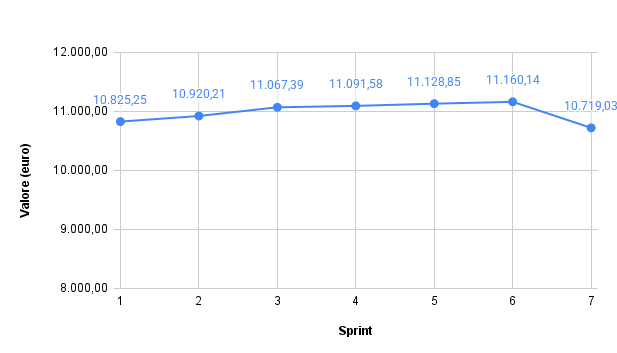
\includegraphics[width=0.75\textwidth]{../graficiMetriche/EAC.png}
    \caption{Andamento del valore di Estimated at Completion (EAC) nella fase RTB}
\end{figure}

\textbf{RTB:} L'analisi dell'Estimated at Completion (EAC) mostra un andamento che si è mantenuto costantemente al di sotto del preventivo totale iniziale (Budget at Completion, pari a 11.395 euro) per tutta la durata della fase. Nonostante alcune fluttuazioni iniziali e i rallentamenti temporali registrati negli \gls{Sprint} 3 e 5, l'ottima efficienza sui costi mantenuta dal team (CPI sempre $\ge$ 1) ha permesso di stabilizzare la stima finale verso il basso. Il gruppo chiude quindi la fase RTB con una proiezione economica solida, confermando l'assenza di rischi legati allo sforamento del budget assegnato.

\newpage
\subsubsection{Planned Value (PV) e Earned Value (EV)}
% [GRAFICO CON LE DUE LINEE PV ED EV]
\begin{figure}[H]
    \centering
    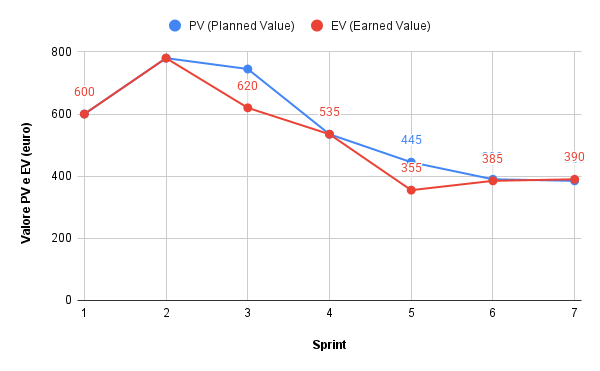
\includegraphics[width=0.75\textwidth]{../graficiMetriche/PV.png}
    \caption{Andamento e confronto di PV e EV nella fase RTB}
\end{figure}

\textbf{RTB:} Dal confronto tra le curve di Planned Value (costo pianificato) ed Earned Value (valore prodotto), emerge una flessione dell'EV durante lo \gls{Sprint} 3 e lo \gls{Sprint} 5 a causa della ridotta disponibilità oraria durante il periodo natalizio e per gli esami invernali.

Tuttavia, analizzando anche l'Actual Cost (AC, non rappresentato in figura ma rendicontato nei consuntivi), emerge che i costi effettivi si sono mantenuti sempre allineati o inferiori all'EV: questo dimostra che le spese sono state costantemente sotto controllo e proporzionate al lavoro realmente svolto, senza alcuno spreco. Durante gli \gls{Sprint} 6 e 7 il team ha incrementato la produttività, riportando l'EV ad allinearsi al PV e chiudendo la fase senza debiti temporali e con un risparmio effettivo (AC $<$ PV).

\newpage
\subsubsection{Schedule Performance Index (SPI)}
% [GRAFICO DELL'SPI]
\begin{figure}[H]
    \centering
    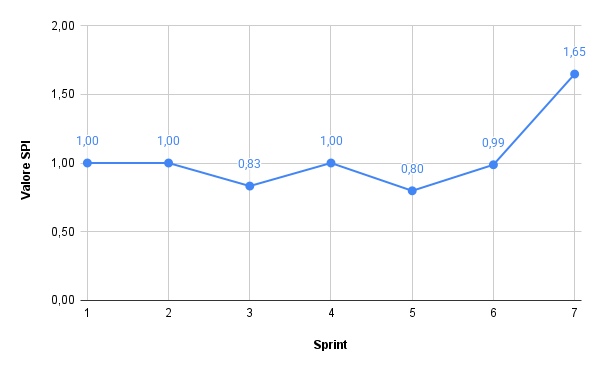
\includegraphics[width=0.75\textwidth]{../graficiMetriche/SPI.png}
    \caption{Andamento dello Schedule Performance Index (SPI) nella fase RTB}
\end{figure}

\textbf{RTB:} L'indice di efficienza della schedulazione (SPI) evidenzia visibilmente l'impatto della sessione d'esami, toccando un picco negativo di 0.83 nello \gls{Sprint} 3 e di 0.80 nello \gls{Sprint} 5. Questo scostamento si è tradotto in una Schedule Variance (SV) negativa, che ha toccato un picco di -125 € nello \gls{Sprint} 3.

Tuttavia, la ridistribuzione dei carichi di lavoro ha permesso di recuperare il gap già negli \gls{Sprint} successivi (4 e 6) e di chiudere lo \gls{Sprint} 7 in perfetto orario (SPI a 1.65) e con un saldo temporale tornato in positivo. L'andamento a "V" del grafico dimostra un'ottima capacità di reazione del team agli imprevisti temporali. L'obiettivo del team è rendere l'indice più stabile nella prossima fase di PB attraverso una migliore pianificazione delle attività.

\newpage
\subsubsection{Cost Performance Index (CPI)}
% [GRAFICO DEL CPI]
\begin{figure}[H]
    \centering
    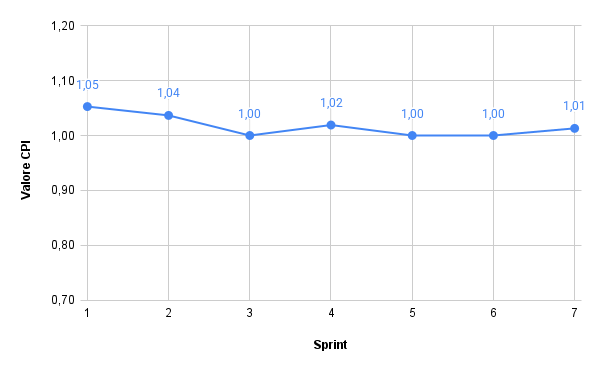
\includegraphics[width=0.75\textwidth]{../graficiMetriche/CPI.png}
    \caption{Andamento del Cost Performance Index (CPI) nella fase RTB}
\end{figure}

\textbf{RTB:} L'indice di efficienza dei costi (CPI) mostra un andamento eccellente, mantenendosi costantemente attorno al valore 1.0 o superiore. Ciò significa che per ogni euro speso dal progetto, il valore prodotto è stato pari o superiore a un euro. Nonostante il ritardo temporale (SPI $<$ 1) negli \gls{Sprint} 3 e 5, il gruppo è stato molto efficiente economicamente: le ore lavorate sono state produttive e non ci sono stati sprechi di risorse o rilavorazioni costose che avrebbero abbassato il CPI.

\newpage
\subsubsection{Cost Variance (CV)}
% [GRAFICO DELLA CV]
\begin{figure}[H]
    \centering
    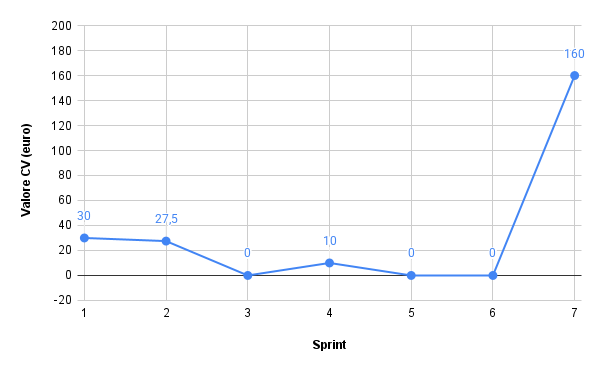
\includegraphics[width=0.75\textwidth]{../graficiMetriche/CV.png}
    \caption{Andamento della Cost Variance (CV) nella fase RTB}
\end{figure}

\textbf{RTB:} La varianza dei costi (CV), calcolata come differenza tra Earned Value e Actual Cost ($EV - AC$), si è mantenuta positiva o prossima allo zero per tutta la durata della fase. Questo indicatore conferma che il gruppo non ha mai speso più del valore generato. Al termine della RTB, il risparmio cumulato è pari a 227,50 €, garantendo al progetto un prezioso margine di sicurezza economico da investire nella successiva fase di Product Baseline.

\newpage
\subsubsection{Requirements Stability Index (RSI)}
% [GRAFICO RSI]
\begin{figure}[H]
    \centering
    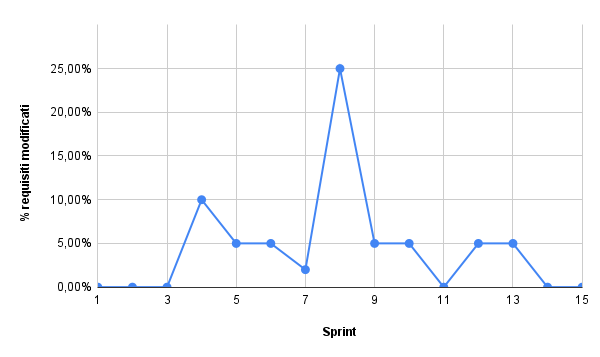
\includegraphics[width=0.75\textwidth]{../graficiMetriche/RSI.png}
    \caption{Andamento del Requirements Stability Index (RSI) nella fase RTB}
\end{figure}

\textbf{RTB:} L'indice di stabilità dei requisiti ha subito alcune variazioni in particolare durante lo \gls{Sprint} 4 e 5. A seguito del colloquio di \gls{verifica} con il prof. Cardin, il gruppo ha dovuto apportare correzioni e raffinamenti ai casi d'uso e ai requisiti precedentemente individuati. Negli ultimi \gls{sprint} (\gls{Sprint} 6), con il consolidamento dell'architettura per il PoC, l'indice si è stabilizzato, indicando che il perimetro del progetto è ora ben definito.

\newpage
\subsubsection{Rischi Non Calcolati (RNC)}
% [GRAFICO RNC]
\begin{figure}[H]
    \centering
    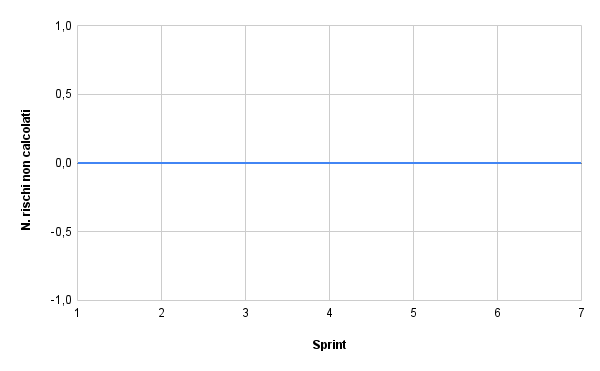
\includegraphics[width=0.75\textwidth]{../graficiMetriche/RNC.png}
    \caption{Numero di rischi non calcolati (RNC) nella fase RTB}
\end{figure}

\textbf{RTB:} Durante la fase RTB, il numero di rischi imprevisti è stato pari a zero (o molto basso). Le principali criticità riscontrate, come la ridotta disponibilità dovuta agli esami (RO-1) e le difficoltà di apprendimento delle tecnologie LLM (RT-1), erano state correttamente previste e mitigate. Il gruppo può ritenersi soddisfatto della capacità di previsione e gestione dei rischi.

\newpage
\subsubsection{Metriche Soddisfatte (MS)}
% [GRAFICO MS]
\begin{figure}[H]
    \centering
    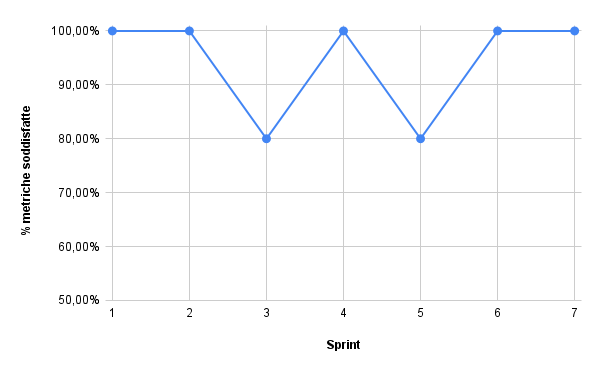
\includegraphics[width=0.75\textwidth]{../graficiMetriche/MS.png}
    \caption{Percentuale delle metriche soddisfatte (MS) nella fase RTB}
\end{figure}

\textbf{RTB:} La percentuale complessiva di metriche soddisfatte ha registrato due flessioni (attorno all'80\%) in corrispondenza degli \gls{Sprint} 3 e 5, principalmente a causa degli sforamenti temporali (SPI < 0.90). Tuttavia, la tenuta impeccabile delle metriche economiche (CPI, CV sempre ottimali) e il recupero finale hanno permesso di chiudere la fase con il 100\% degli indicatori in stato accettabile o ottimale. Il processo adottato è pertanto ritenuto maturo e validato.

\end{document}
